% questions.tex —— 1985 年·全国卷·理科 · 题目内容片段（无答案）
% 由 tools/generate_projects.py 依来源总账自 1985/1985_数学真题_全国理_试题.md 生成，勿手改（改源 MD 后重跑）


\gkpart{理科数学}

\begin{gktip}
\textbf{来源说明}：本题面依据固定源 PDF《1985 全国理科数学》单页逐题转录。固定源为一页完整题面，原卷页码为 25；该 PDF 不含答案页，下列答案和解析由本库独立推导，不声称代表官方发布版本。
\end{gktip}

\begin{question}
\gkti{1}如果正方体 $ABCD-A'B'C'D'$ 的棱长为 $a$，那么四面体 $A'-ABD$ 的体积是\mbox{（　　）}

\nopagebreak[4]
\[
\text{（A）}\ \frac{a^3}{2}
\qquad
\text{（B）}\ \frac{a^3}{3}
\qquad
\text{（C）}\ \frac{a^3}{4}
\qquad
\text{（D）}\ \frac{a^3}{6}
\]

\end{question}
\begin{question}
\gkti{2}$\tan x=1$ 是 $x=\dfrac54\pi$ 的\mbox{（　　）}

（A）必要条件　　（B）充分条件　　（C）充分必要条件　　（D）既不充分又不必要的条件

\end{question}
\begin{question}
\gkti{3}在下面给出的函数中，哪一个函数既是区间 $\left(0,\dfrac\pi2\right)$ 上的增函数又是以 $\pi$ 为周期的偶函数\mbox{（　　）}

（A）$y=x^2\ (x\in\mathbb R)$

（B）$y=|\sin x|\ (x\in\mathbb R)$

（C）$y=\cos2x\ (x\in\mathbb R)$

（D）$y=e^{\sin2x}\ (x\in\mathbb R)$

\Needspace{0.4\textheight}
\end{question}
\begin{question}
\gkti{4}极坐标方程

\nopagebreak[4]
\[
\rho=a\sin\theta\qquad(a>0)
\]

的图象是\mbox{（　　）}
\nopagebreak[4]
\begin{center}% 1985 年全国卷理科第 4 题：极坐标方程 rho=a sin(theta) 的四个选项
\begin{tikzpicture}[scale=0.62,>=stealth]
  \begin{scope}[shift={(0,1.55)}]
    \draw[->] (-1.15,0)--(1.65,0) node[right] {$x$};
    \node[above left] at (-1.0,0.02) {$O$};
    \draw (0.34,0) circle (0.78);
    \fill (0.34,0) circle (1pt) node[below] {$\frac a2$};
    \node[below] at (0,-1.15) {（A）};
  \end{scope}
  \begin{scope}[shift={(3.0,1.55)}]
    \draw[->] (-1.15,0)--(1.65,0) node[right] {$x$};
    \node[above left] at (-1.0,0.02) {$O$};
    \draw (0.75,0) circle (1.12);
    \fill (0.75,0) circle (1pt) node[below] {$a$};
    \node[below] at (0,-1.15) {（B）};
  \end{scope}
  \begin{scope}[shift={(0,-1.55)}]
    \draw[->] (-1.15,0)--(1.65,0) node[right] {$x$};
    \node[above left] at (-1.0,0.02) {$O$};
    \draw (0,0.78) circle (0.78);
    \fill (0,0.78) circle (1pt) node[right] {$\frac a2$};
    \draw (0,0)--(0,0.78);
    \node[below] at (0,-1.15) {（C）};
  \end{scope}
  \begin{scope}[shift={(3.0,-1.55)}]
    \draw[->] (-1.15,0)--(1.65,0) node[right] {$x$};
    \node[above left] at (-1.0,0.02) {$O$};
    \draw (0,1.05) circle (1.05);
    \fill (0,1.05) circle (1pt) node[right] {$a$};
    \draw (0,0)--(0,1.05);
    \node[below] at (0,-1.15) {（D）};
  \end{scope}
\end{tikzpicture}
\end{center}
\nopagebreak[4]
\end{question}
\begin{question}
\gkti{5}用 $1,2,3,4,5$ 这五个数字，可以组成比 $20000$ 大，并且百位数不是数字 $3$ 的没有重复数字的五位数，共有\mbox{（　　）}

（A）96 个　　（B）78 个　　（C）72 个　　（D）64 个

\end{question}
\begin{question}
\gkti{6}求方程

\nopagebreak[4]
\[
2\sin\left(x+\frac\pi6\right)=1
\]

的解集。

\end{question}
\begin{question}
\gkti{7}设 $|a|\le1$，求

\nopagebreak[4]
\[
\arccos a+\arccos(-a)
\]

的值。

\end{question}
\begin{question}
\gkti{8}求曲线

\nopagebreak[4]
\[
y^2=-16x+64
\]

的焦点。

\end{question}
\begin{question}
\gkti{9}设

\nopagebreak[4]
\[
(3x-1)^6=a_6x^6+a_5x^5+a_4x^4+a_3x^3+a_2x^2+a_1x+a_0,
\]

求 $a_6+a_5+a_4+a_3+a_2+a_1+a_0$ 的值。

\end{question}
\begin{question}
\gkti{10}设函数 $f(x)$ 的定义域是 $[0,1]$，求函数 $f(x^2)$ 的定义域。

\end{question}
\begin{question}
\gkti{11}解方程：

\nopagebreak[4]
\[
\log_4(3-x)+\log_{0.25}(3+x)
=\log_4(1-x)+\log_{0.25}(2x+1).
\]

\end{question}
\begin{question}
\gkti{12}解不等式：

\nopagebreak[4]
\[
\sqrt{2x+5}>x+1.
\]

\Needspace{0.4\textheight}
\end{question}
\begin{question}
\gkti{13}如图，设平面 $AC$ 和 $BD$ 相交于 $BC$，它们所成的一个二面角为 $45^\circ$，$P$ 为平面 $AC$ 内的一点，$Q$ 为平面 $BD$ 内的一点。已知直线 $MQ$ 是直线 $PQ$ 在平面 $BD$ 内的射影，并且 $M$ 在 $BC$ 上。又设 $PQ$ 与平面 $BD$ 所成的角为 $\beta$，$\angle CMQ=\theta$（$0^\circ<\theta<90^\circ$），线段 $PM$ 的长为 $a$，求线段 $PQ$ 的长。

\begin{gktip}
原源 PDF 第 1 页附有两个相交平面、点 $P,Q,M$ 及投影线段的示意图；LaTeX 版按源图关系重绘。
\end{gktip}
\nopagebreak[4]
\begin{center}% 1985 年全国卷理科第 13 题：两个相交平面及投影关系
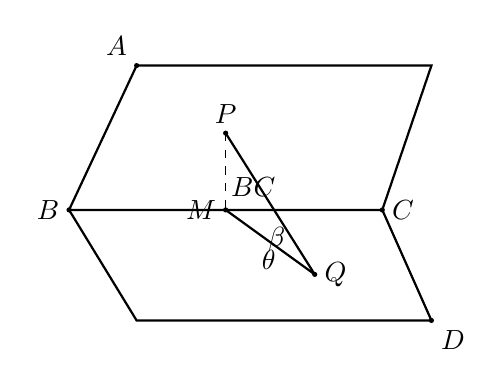
\begin{tikzpicture}[scale=0.78]
  \coordinate (B) at (0,0);
  \coordinate (C) at (5.1,0);
  \coordinate (A) at (1.1,2.35);
  \coordinate (E) at (5.9,2.35);
  \coordinate (F) at (1.1,-1.8);
  \coordinate (D) at (5.9,-1.8);
  \coordinate (P) at (2.55,1.25);
  \coordinate (M) at (2.55,0);
  \coordinate (Q) at (4.0,-1.05);
  \draw[thick] (B)--(A)--(E)--(C)--cycle;
  \draw[thick] (B)--(F)--(D)--(C);
  \draw[thick] (B)--(C);
  \draw[dashed] (P)--(M);
  \draw[thick] (P)--(Q);
  \draw[thick] (M)--(Q);
  \fill (A) circle (1.2pt) node[above left] {$A$};
  \fill (B) circle (1.2pt) node[left] {$B$};
  \fill (C) circle (1.2pt) node[right] {$C$};
  \fill (D) circle (1.2pt) node[below right] {$D$};
  \fill (P) circle (1.2pt) node[above] {$P$};
  \fill (M) circle (1.2pt) node[left] {$M$};
  \fill (Q) circle (1.2pt) node[right] {$Q$};
  \node at (3.0,0.38) {$BC$};
  \node at (3.38,-0.48) {$\beta$};
  \node at (3.25,-0.82) {$\theta$};
\end{tikzpicture}
\end{center}
\nopagebreak[4]
\end{question}
\begin{question}
\gkti{14}设 $O$ 为复平面的原点，$Z_1$ 和 $Z_2$ 为复平面内的两动点，并且满足：

（1） $Z_1$ 和 $Z_2$ 所对应的复数的辐角分别为定值 $\theta$ 和 $-\theta$（$0<\theta<\dfrac\pi2$）；

（2） $\triangle OZ_1Z_2$ 的面积为定值 $S$。

求 $\triangle OZ_1Z_2$ 的重心 $Z$ 所对应的复数的模的最小值。

\Needspace{0.4\textheight}
\end{question}
\begin{question}
\gkti{15}已知两点 $P(-2,2)$、$Q(0,2)$ 以及一条直线

\nopagebreak[4]
\[
L:y=x,
\]

设长为 $\sqrt2$ 的线段 $AB$ 在直线 $L$ 上移动，如图，求直线 $PA$ 和 $QB$ 的交点 $M$ 的轨迹方程。（要求把结果写成普通方程。）

\begin{gktip}
原源 PDF 第 1 页附有 $P,Q$、直线 $y=x$、可动线段 $AB$ 和交点 $M$ 的示意图；LaTeX 版按源图关系重绘。
\end{gktip}
\nopagebreak[4]
\begin{center}% 1985 年全国卷理科第 15 题：线段 AB 在 y=x 上移动
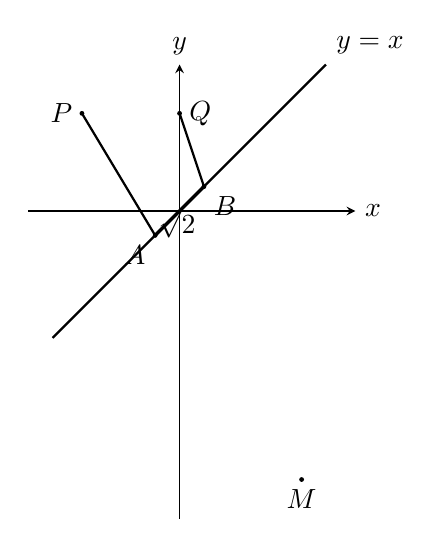
\begin{tikzpicture}[scale=0.62,>=stealth]
  \draw[->] (-3.1,0)--(3.6,0) node[right] {$x$};
  \draw[->] (0,-6.3)--(0,3.0) node[above] {$y$};
  \draw[thick] (-2.6,-2.6)--(3.0,3.0) node[above right] {$y=x$};
  \coordinate (P) at (-2,2);
  \coordinate (Q) at (0,2);
  \coordinate (A) at (-0.5,-0.5);
  \coordinate (B) at (0.5,0.5);
  \coordinate (M) at (2.5,-5.5);
  \draw[thick] (P)--(A);
  \draw[thick] (Q)--(B);
  \draw[very thick] (A)--(B);
  \fill (P) circle (1.4pt) node[left] {$P$};
  \fill (Q) circle (1.4pt) node[right] {$Q$};
  \fill (A) circle (1.4pt) node[below left] {$A$};
  \fill (B) circle (1.4pt) node[below right] {$B$};
  \fill (M) circle (1.4pt) node[below] {$M$};
  \node at (-0.05,-0.25) {$\sqrt2$};
\end{tikzpicture}
\end{center}
\nopagebreak[4]
\end{question}
\begin{question}
\gkti{16}设

\nopagebreak[4]
\[
a_n=\sqrt{1\cdot2}+\sqrt{2\cdot3}+\cdots+\sqrt{n(n+1)}
\qquad(n=1,2,\ldots).
\]

\Needspace{5\baselineskip}
（1） 证明：不等式

\nopagebreak[4]
\[
\frac{n(n+1)}2<a_n<\frac{(n+1)^2}{2}
\]

对所有的正整数 $n$ 都成立；

\Needspace{5\baselineskip}
（2） 设

\nopagebreak[4]
\[
b_n=\frac{a_n}{n(n+1)}
\qquad(n=1,2,\ldots),
\]

\Needspace{5\baselineskip}
用定义证明：

\nopagebreak[4]
\[
\lim_{n\to\infty}b_n=\frac12.
\]

\end{question}
\begin{question}
\gkti{17}设 $a\text{、}b$ 是两个实数，

\nopagebreak[4]
\[
A=\{(x,y)\mid x=n,\ y=na+b,\ n\text{ \text{是整数}}\},
\]

\nopagebreak[4]
\[
B=\{(x,y)\mid x=m,\ y=3m^2+15,\ m\text{ \text{是整数}}\},
\]

\nopagebreak[4]
\[
C=\{(x,y)\mid x^2+y^2\le144\}
\]

是平面 $xOy$ 内的点集合，讨论是否存在 $a$ 和 $b$ 使得

（1） $A\cap B\ne\varnothing$（$\varnothing$ 表示空集），

（2） $(a,b)\in C$

同时成立。

\end{question}
\begin{question}
\gkti{18}已知曲线

\nopagebreak[4]
\[
y=x^3-6x^2+11x-6.
\]

在它对应于 $x\in[0,2]$ 的弧段上求一点 $P$，使得曲线在该点的切线在 $y$ 轴上的截距为最小，并求出这个最小值。

\end{question}